%% Submissions for peer-review must enable line-numbering
%% using the lineno option in the \documentclass command.
%%
%% Preprints and camera-ready submissions do not need
%% line numbers, and should have this option removed.
%%
%% Please note that the line numbering option requires
%% version 1.1 or newer of the wlpeerj.cls file, and
%% the corresponding author info requires v1.2

\documentclass[fleqn,10pt,lineno]{wlpeerj} % for journal submissions

% ZNK -- Adding headers for pandoc

\setlength{\emergencystretch}{3em}
\providecommand{\tightlist}{
\setlength{\itemsep}{0pt}\setlength{\parskip}{0pt}}
\usepackage[unicode=true]{hyperref}
\usepackage{longtable}


% Pandoc syntax highlighting
% See https://github.com/rstudio/rticles/issues/182

% Pandoc citation processing
\newlength{\csllabelwidth}
\setlength{\csllabelwidth}{3em}
\newlength{\cslhangindent}
\setlength{\cslhangindent}{1.5em}
% for Pandoc 2.8 to 2.10.1
\newenvironment{cslreferences}%
  {}%
  {\par}
% For Pandoc 2.11+
\newenvironment{CSLReferences}[2] % #1 hanging-ident, #2 entry spacing
 {% don't indent paragraphs
  \setlength{\parindent}{0pt}
  % turn on hanging indent if param 1 is 1
  \ifodd #1 \everypar{\setlength{\hangindent}{\cslhangindent}}\ignorespaces\fi
  % set entry spacing
  \ifnum #2 > 0
  \setlength{\parskip}{#2\baselineskip}
  \fi
 }%
 {}
\usepackage{calc} % for calculating minipage widths
\newcommand{\CSLBlock}[1]{#1\hfill\break}
\newcommand{\CSLLeftMargin}[1]{\parbox[t]{\csllabelwidth}{#1}}
\newcommand{\CSLRightInline}[1]{\parbox[t]{\linewidth - \csllabelwidth}{#1}\break}
\newcommand{\CSLIndent}[1]{\hspace{\cslhangindent}#1}

% Pandoc Header
\usepackage{float}
\usepackage[tablesfirst, heads, nolists, nomarkers]{endfloat}
\usepackage{booktabs}
\usepackage{longtable}
\usepackage{array}
\usepackage{multirow}
\usepackage{wrapfig}
\usepackage{float}
\usepackage{colortbl}
\usepackage{pdflscape}
\usepackage{tabu}
\usepackage{threeparttable}
\usepackage{threeparttablex}
\usepackage[normalem]{ulem}
\usepackage{makecell}
\usepackage{xcolor}

\title{Urban biogeography of fungal endophytes across San Francisco}

\author[1]{Emma Gibson}

\author[1]{Naupaka Zimmerman}

\corrauthor[1]{Naupaka Zimmerman}{\href{mailto:nzimmerman@usfca.edu}{\nolinkurl{nzimmerman@usfca.edu}}}

\affil[1]{Department of Biology, University of San Francisco}


%
% \author[1]{First Author}
% \author[2]{Second Author}
% \affil[1]{Address of first author}
% \affil[2]{Address of second author}
% \corrauthor[1]{First Author}{f.author@email.com}

% 

\begin{abstract}
In natural and agricultural systems, the plant microbiome--the microbial organisms associated with plant tissues--has been shown to have important effects on host physiology and ecology, yet we know little about how these plant-microbe relationships play out in urban environments. Here we characterize the composition of fungal communities associated with leaves of one of the most common sidewalk trees in the city of San Francisco, California. We focus our efforts on endophytic fungi (asymptomatic microfungi that live inside healthy leaves), which have been shown in other systems to have large ecological effects on the health of their plant hosts. Specifically, we characterized the foliar fungal microbiome of \emph{Metrosideros excelsa} (Myrtaceae) trees growing in a variety of urban environmental conditions. We used high-throughput culturing, PCR, and Sanger sequencing of the ITS nrDNA region to quantify the composition and structure of fungal communities growing within healthy leaves of 30 \emph{M. excelsa} trees from 6 distinct sites, which were selected to capture the range of environmental conditions found within city limits. Sequencing resulted in 854 high-quality ITS sequences. These sequences clustered into 85 Operational Taxonomic Units (97\% VSEARCH OTUs). We found that these communities encompass relatively high alpha (within) and beta (between-site) diversity. Because the communities are all from the same host tree species, and located in relatively close geographical proximity to one another, these analyses suggest that urban environmental factors such as heat islands or differences in vegetation or traffic density (and associated air quality) may potentially be influencing the composition of these fungal communities. These biogeographic patterns provide evidence that plant microbiomes in urban environments can be as dynamic and complex as their natural counterparts. As human populations continue to transition out of rural areas and into cities, understanding the factors that shape environmental microbial communities in urban ecosystems stands to become increasingly important.
% Dummy abstract text. Dummy abstract text. Dummy abstract text. Dummy abstract text. Dummy abstract text. Dummy abstract text. Dummy abstract text. Dummy abstract text. Dummy abstract text. Dummy abstract text. Dummy abstract text.
\end{abstract}

\begin{document}

\flushbottom
\maketitle
\thispagestyle{empty}

\begin{table}[!h]

\caption{\label{tab:class-abundance-table}Overall sequenced fungal isolate counts by Class and Order. All fungi successfully  sequenced in this study were placed within the Ascomycota.}
\centering
\begin{tabular}[t]{llr}
\toprule
Class & Order & Number of sequences\\
\midrule
Dothideomycetes & Capnodiales & 266\\
Dothideomycetes & Botryosphaeriales & 127\\
Dothideomycetes & Pleosporales & 52\\
Dothideomycetes & unclassified,Capnodiales & 3\\
Dothideomycetes & Trypetheliales & 1\\
Dothideomycetes & unclassified & 1\\
\addlinespace
Eurotiomycetes & Eurotiales & 57\\
\addlinespace
Leotiomycetes & Helotiales & 19\\
\addlinespace
Pezizomycetes & Pezizales & 54\\
\addlinespace
Sordariomycetes & Xylariales & 237\\
Sordariomycetes & Diaporthales & 49\\
Sordariomycetes & Coniochaetales & 38\\
Sordariomycetes & Sordariales & 9\\
Sordariomycetes & Hypocreales & 7\\
Sordariomycetes & Glomerellales & 1\\
\bottomrule
\end{tabular}
\end{table}

\begin{figure}[p!]
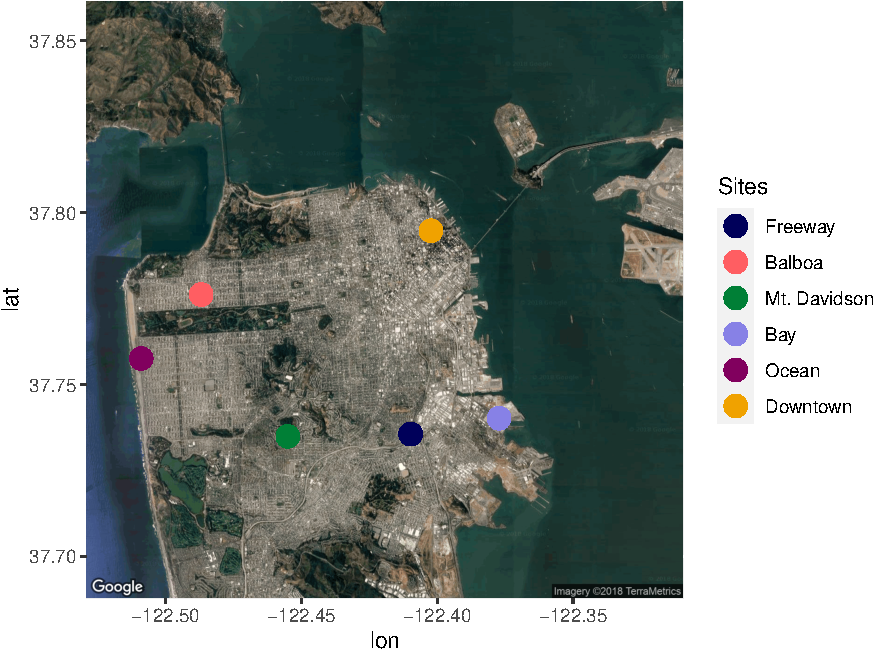
\includegraphics{gibson2021_files/figure-latex/site-map-1} \caption{A map of the locations sampled across the city of San Francisco, California, USA. Five trees from each site were sampled. Sites were selected to span the range of environmental conditions across the city. Map data © 2021 Google.}\label{fig:site-map}
\end{figure}

\begin{figure}
\centering
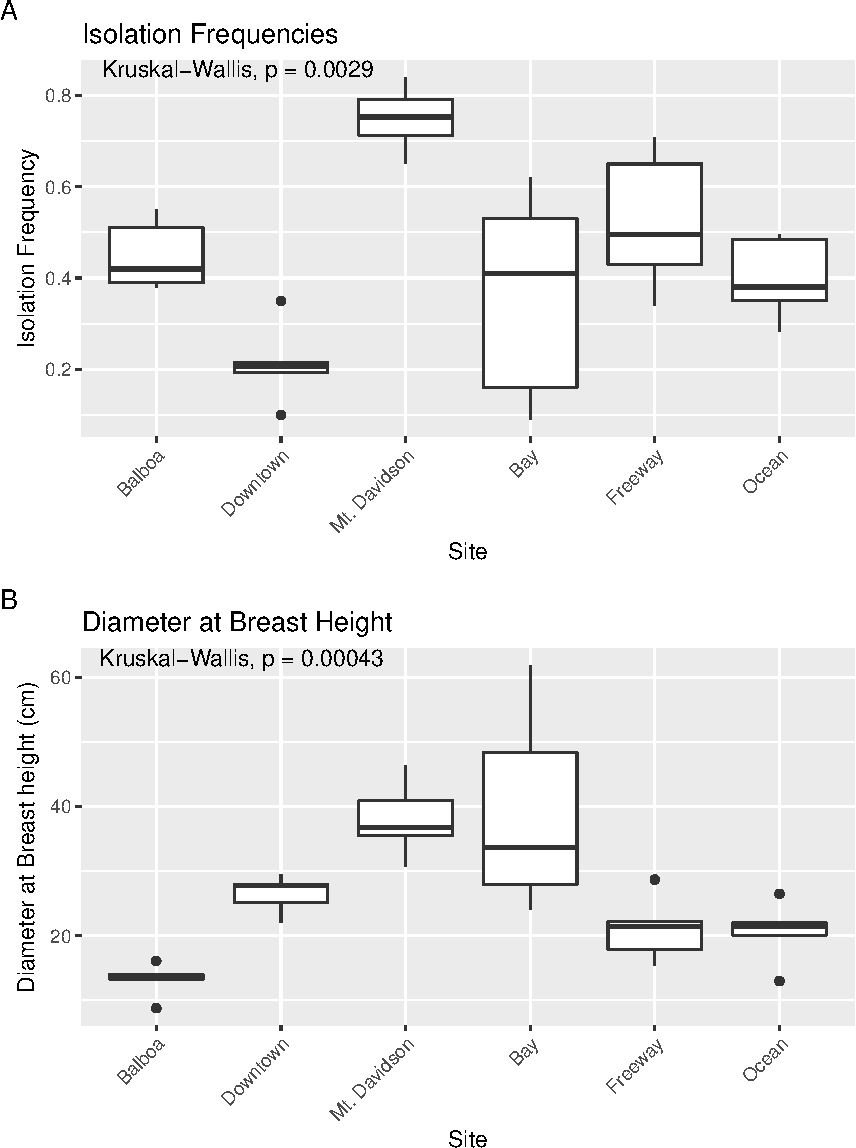
\includegraphics{gibson2021_files/figure-latex/isolation-dbh-freq-plots-1.pdf}
\caption{\label{fig:isolation-dbh-freq-plots}Isolation frequencies (A) and tree diameters (B) at each site. Isolation frequency (A) is a measure of how many slant tubes showed signs of fungal growth, out of how many total slant tubes were made. Approximately 100 slant tubes were made for each tree except for the trees in the downtown site, which had 140 slant tubes per tree because they had low isolation frequencies during the initial sampling. Sites along x axis are arranged left to right in order of their geographic location from west (left) to east (right).}
\end{figure}

\begin{figure}
\centering
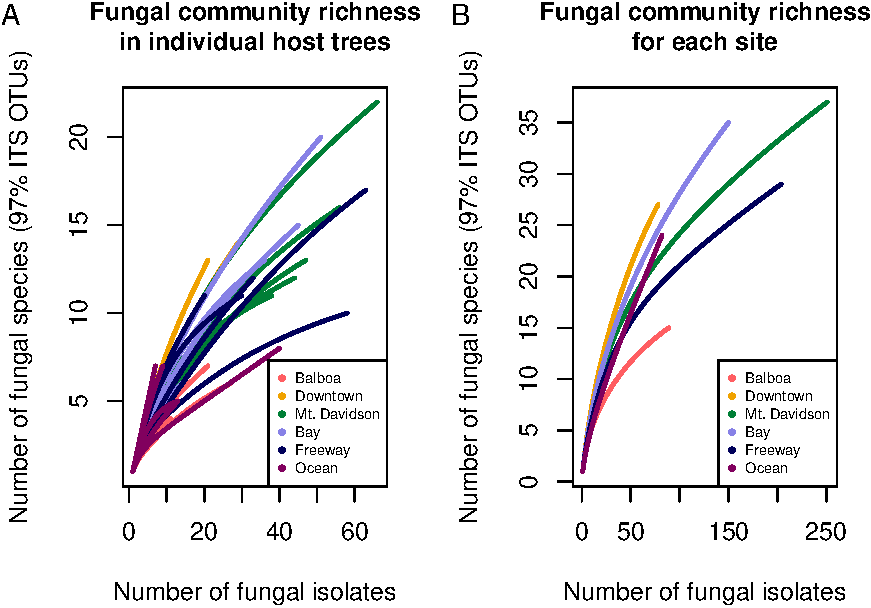
\includegraphics{gibson2021_files/figure-latex/rarefaction-plot-1.pdf}
\caption{\label{fig:rarefaction-plot}Species accumulation curves showing fungal community OTU richness. Each line in A represents the OTU richness for a single host tree. Each line in B represents the combined OTU richness of all trees (n = 5) in one site.}
\end{figure}

\begin{figure}
\centering
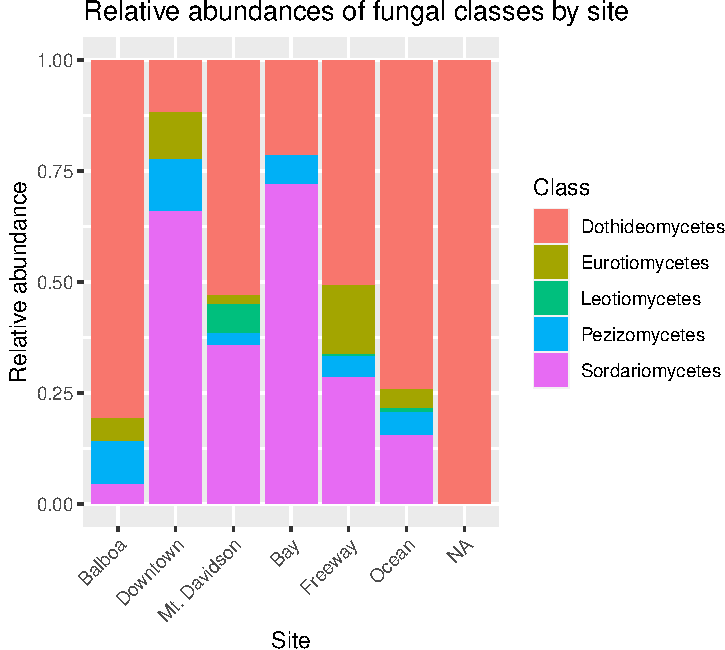
\includegraphics{gibson2021_files/figure-latex/taxonomy-by-site-plot-1.pdf}
\caption{\label{fig:taxonomy-by-site-plot}Normalized relative abundances of taxonomic groupings (Classes in A and Orders in B) in each site. Sites along x axis are arranged left to right in order of their geographic location from west (left) to east (right).}
\end{figure}

\begin{figure}
\centering
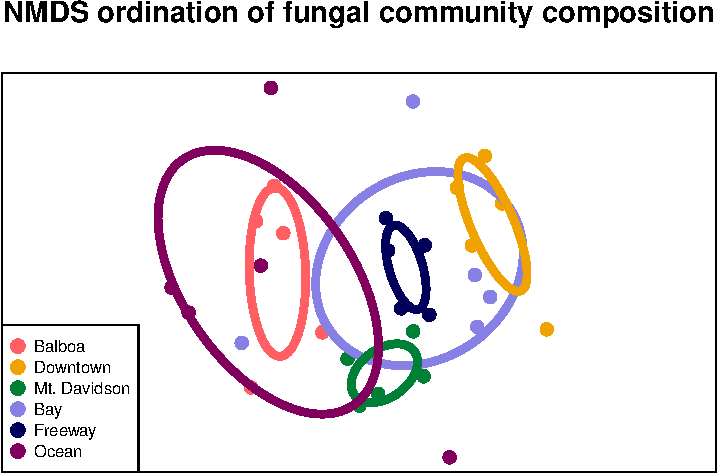
\includegraphics{gibson2021_files/figure-latex/nmds-plot-1.pdf}
\caption{\label{fig:nmds-plot}NMDS ordination of community compositions. Each point represents the endophytic community of one tree, and the size of the point corresponds to that tree's DBH, while the color of said point corresponds to the site that tree is from. Points that are closer together indicate that the trees they represent have similar community compositions. The ellipses show the standard error around the centroid of all points within a site, and are also color-coded according to which site they represent.}
\end{figure}

\begin{table}[!h]

\caption{\label{tab:permanova-table}PERMANOVA model output based on Bray-Curtis distance, with permutations stratified by site. Foliar fungal community composition in leaves of \emph{Metrosideros excelsa} across San Francisco is significantly related to both site of sampling and tree diameter at breast height (DBH).}
\centering
\begin{tabular}[t]{lrrrrrr}
\toprule
Term & df & Sum of Squares & Mean of Squares & F & R\textasciicircum{}2 & p-value\\
\midrule
trees\$Site\_ID & 5 & 3.642 & 0.728 & 3.015 & 0.373 & 0.022\\
trees\$DBH\_cm & 1 & 0.556 & 0.556 & 2.302 & 0.057 & 0.022\\
Residuals & 23 & 5.557 & 0.242 & NA & 0.570 & NA\\
Total & 29 & 9.755 & NA & NA & 1.000 & NA\\
\bottomrule
\end{tabular}
\end{table}

\hypertarget{introduction}{%
\section*{Introduction}\label{introduction}}
\addcontentsline{toc}{section}{Introduction}

Although major cities and urban centers only cover a small portion the Earth's total geographic area, more than 50\% of the human population lives in these urban centers, and the impact that these cities have on the environment can be seen worldwide (Schneider, Friedl, and Potere 2009). With increasing urbanization, understanding the ecology of cities and urban settings has become critical to human health and well being. Despite their comparatively small geographic size, the high density of human populations in these environments makes them distinct ecosystems with their own unique dynamics (Sukopp 1998). Urban environments represent the convergence of humans from around the world, any plant or animal species those humans might have brought with them, and infrastructures such as roads, sewers, and tall buildings. Despite the complexity that these ecosystems present, they are often overlooked by ecologists because more traditional ecology has focused on `natural' systems. In urban systems, however, human influence is a primary ecological factor (McDonnell and Niemelä 2011). In recent years, ecologists have begun studying the urban environment just as they would a natural environment, in order to understand the novel environmental conditions this setting presents to the organisms that live there (Wu 2014).

In this study, we focus on the urban ecology of trees in San Francisco, California. Urban trees can play a major role in shaping the ecosystem of a city. Just as the trees in a forest have a considerable impact on its climate and ecology, trees in cities can have notable effects on a city's environment. For example, plant life in cities can impact temperature, air quality, and other aspects of human health (Willis and Petrokofsky 2017). The urban heat island effect, which occurs when `islands' of heat form as heat gets trapped between tall buildings, is one of the most well-documented unique urban anthropogenic environmental conditions (Oke 1973). Trees in urban environments have been shown to interact with these city-specific environmental factors (Kong et al. 2014). For example, trees in cities have been shown to improve urban air quality by taking up significant amounts of carbon dioxide from city air (Nowak et al. 2014). As pollution generated in urban centers is one of the major contributing factors to worldwide pollution, trees in urban environments may have a role in managing the environmental impacts of urbanization (Alberti et al. 2003).

Due to their importance, there is growing interest in understanding and maintaining sustainable urban ecologies. One potentially major factor influencing health of plants both in nature and cities is the plant microbiome. As the widespread availability of DNA sequencing has made it possible to characterize microbial communities more easily and comprehensively, the microbiome has become a major area of interest in numerous organisms (Kyrpides, Eloe-Fadrosh, and Ivanova 2016). Just as the emerging field of human microbiome study has revealed that symbiotic, non-pathogenic microbes can have major impacts on human health (David et al. 2014), plants also host numerous symbiotic microbes. Similar to the human microbiome, the plant microbiome contains great diversity and is comprised of multiple distinct communities in various tissue systems such as the roots (rhizosphere), leaf surface (phyllosphere), and leaf interior (endosphere) (Turner, James, and Poole 2013). All of these microbiomes can have an impact on their host's physiology. For instance, bacterial root microbes have been shown to play a role in the growth of various plant species (Gaiero et al. 2013). They can also play a variety of roles in host physiology, depending on their location within the plant (Schlaeppi and Bulgarelli 2015). These communities can be quite dynamic, and vary with factors such as plant age (Cavaglieri, Orlando, and Etcheverry 2009). While each of these sets of interactions is important, here we focus on the microbial ecology of fungal microorganisms living in the leaf endosphere. The endosphere is an ideal system for biogeographic studies, both because it is highly diverse, well replicated, and because it is a major interface between the host plant and its environment (Meyer and Leveau 2012).

Endophytic microbes are naturally found in the interior of leaves, whether introduced by natural wounds or openings in the leaf surface, or through penetrating the plant surface with hydrolytic enzymes (Hallmann et al. 1997). Although some of these microbes may be latent pathogens or decomposers waiting for the leaf to die, others are mutualists that may confer a benefit to their host (Carroll 1988). In wild grasses, symbiotic fungi have been shown to protect their hosts by discouraging herbivory, and can even affect host reproductive viability in those same systems (Clay 1988). In controlled settings, inoculation experiments have shown that specific species of endophytes can have an impact on their host's overall health, including factors such as resistance and susceptibility to disease (Busby, Ridout, and Newcombe 2016). In nature, the fungal microbial communities can have impacts on their host's physiology, such as limiting pathogen damage (Arnold et al. 2003).

In the wild, endophytic communities display species diversity comparable to that of any macroscopic community, even among individual trees from the same species (Gazis, Rehner, and Chaverri 2011). However, determining the factors that influence this diversity across disparate environments remains an area of active research. The biodiversity of these communities can be quite high, especially in areas like tropical forests (Arnold and Lutzoni 2007). In such natural settings, plant-associated microbial community compositions can show clear biogeographic structure (Andrews and Harris 2000). The urban setting, however, may be distinct, because factors such as rainfall and elevation will likely be less apparent over a smaller geographic area, even as new factors such as proximity to roads and tall buildings may introduce effects of their own. Studies of suburban forests in Japan have indicated that an urban setting has a notable impact on endophytic diversity (Matsumura and Fukuda 2013). However, the full impact of urban environmental factors on endophytic communities has yet to be completely understood.

In this study, we used culturing and barcode gene sequencing to identify the species makeup of endophytic communities in the New Zealand Christmas Tree (Māori: pōhutukawa), \emph{Metrosideros excelsa} (Myrtaceae), throughout San Francisco, CA, to quantify the diversity and biogeographic patterns of foliar fungal communities in this urban environment. Based on studies in natural systems, we expected to find high community diversity both within and between sites, as well as a degree of biogeographic structure to these community compositions. We also anticipated that urban environmental factors might play a role in shaping the biogeography in these endophytic communities. We found that leaves from trees sampled at different sites across the city did indeed harbor distinct communities, and also that culture-based fungal isolation frequencies differed among sites as well.

\hypertarget{methods}{%
\section*{Methods}\label{methods}}
\addcontentsline{toc}{section}{Methods}

\hypertarget{host-selection}{%
\subsection*{Host Selection}\label{host-selection}}
\addcontentsline{toc}{subsection}{Host Selection}

We chose to focus on \emph{Metrosideros excelsa} as a focal host tree. \emph{Metrosideros excelsa} is widely planted throughout San Francisco and as such we were able to obtain samples from a large number of trees in a variety of locations throughout the city. Although \emph{M. excelsa's} endophytic communities have been characterized in its native range (New Zealand), there have been few studies about these communities outside of its native environment or in an urban setting (McKenzie, Buchanan, and Johnston 1999). In a Hawaiian endemic congener, \emph{Metrosideros polymorpha}, the species makeup of foliar fungal endophyte communities has been shown to vary greatly across gradients of environmental factors such as elevation and rainfall (Zimmerman and Vitousek 2012).

\hypertarget{site-selection}{%
\subsection*{Site Selection}\label{site-selection}}
\addcontentsline{toc}{subsection}{Site Selection}

We selected six sites across the city for leaf sample collection (Fig. \ref{fig:site-map}). When selecting sites, we took factors such as traffic levels, estimated temperature, proximity to tall buildings, elevation, and proximity to the ocean and San Francisco Bay into account. In selecting the sites, we wanted to capture the wide range of potential urban climates. We used street tree location data available from the City of San Francisco (permalink: \url{https://data.sfgov.org/City-Infrastructure/Street-Tree-List/tkzw-k3nq}), which documents the location and species of every tree in San Francisco, to choose unique locations around the city with sufficient densities of \emph{Metrosideros excelsa} individuals (Fig. \ref{fig:site-map}).

\hypertarget{sample-collection}{%
\subsection*{Sample Collection}\label{sample-collection}}
\addcontentsline{toc}{subsection}{Sample Collection}

We collected small branches from 5 trees in each of these sites using a clipper pole, collecting at least 3 sun-exposed outer branches from each tree. Because \emph{M. excelsa} is an evergreen tree and the newer leaves are likely to contain fewer fungi, we controlled for leaf age by only collecting branches which contained dark green leaves that appeared to be at least one year old. We collected all samples on the same day, August 26, 2017, to ensure that daily weather patterns and seasonal effects would not have an impact on the microbial community composition. Once collected, leaves were stored in labeled plastic bags and stored at 4\(^{\circ}\)C until culturing. All leaves were processed within 48 hours of collection. Permission to sample leaves was granted by the San Francisco Bureau of Urban Forestry.

\hypertarget{culturing-methods}{%
\subsection*{Culturing Methods}\label{culturing-methods}}
\addcontentsline{toc}{subsection}{Culturing Methods}

From each sample, we selected a subset of dark green asymptomatic leaves for culturing. We surface-sterilized the leaves by first rinsing them with distilled water, then immersing them in a sterile petri dish with 95\% ethanol for 10 seconds, 0.5\% NaOCl for 2 minutes, then 70\% ethanol for another 2 minutes following Arnold et al. (2007). We emptied the dish between rinses and left it closed until inside a sterile biosafety cabinet after the last rinse. We then cut the leaves into small (2mm x 2mm) pieces with flame-sterilized scissors and placed them into 1.5 mL microcentrifuge slant tubes partially filled with 2\% VWR-brand malt extract agar (MEA). For each tree, we prepared 6 leaves and made 100 tubes, except for the trees from the downtown site. For the trees at this site, we prepared 140 tubes per tree because we found that they had low isolation frequencies in a preliminary sampling bout. All leaves were prepared this way within 48 hours of the initial leaf sampling, to prevent death of the leaf tissue from altering the fungal community composition.

After two weeks, we evaluated the tubes for fungal growth and subcultured the emergent fungi from tubes with growth onto 35mm plates with 2\% MEA in order to better evaluate their morphotypes and accumulate sufficient tissue for future barcode gene sequencing and water voucher preparation. We re-evaluated and subcultured these tubes in the following months to capture any late-growing fungi. Each pure culture was vouchered in sterile dI water and stored in a living culture collection in the Zimmerman Lab at the University of San Francisco.

\hypertarget{molecular-methods}{%
\subsection*{Molecular Methods}\label{molecular-methods}}
\addcontentsline{toc}{subsection}{Molecular Methods}

We extracted DNA from fungal mycelium using the Sigma RED Extract `n Amp DNA extraction kit and following previously published protocols (U'Ren et al. 2012). First, we added fungal tissue to sterile tubes filled with 1 mm zirconium oxide beads, then added 100 \(\mu\)L of Extract 'n' Amp DNA extraction solution. Next, we put the tubes in a bead-beater (Mini-Beadbeater-96, Bio Spec Products Inc.) for one minute. The samples were then placed on a heat block at 95\(^{\circ}\)C for 10 minutes. After the heating step, we added a dilution buffer to each tube and stored them at 4\(^{\circ}\)C until PCR.

We performed PCR using fungal-specific primers for the Internal Transcribed Spacer region, a commonly-accepted fungal barcode locus (Schoch et al. 2012), using the ITS1F forward primer (5'-CTT GGT CAT TTA GAG GAA GTA A-3') and ITS4 reverse primer (5'-TCC TCC GCT TAT TGA TAT GC-3'). For each PCR reaction, we used 1 \(\mu\)L of template DNA, 10 \(\mu\)L Extract 'n Amp Taq polymerase, 6.4 \(\mu\)L PCR-grade water, 1 \(\mu\)L bovine serum albumin, 0.8 \(\mu\)L ITS1F forward primer, and 0.8 \(\mu\)L ITS4 reverse primer (U'Ren et al. 2012). For the PCR reaction, we used a BioRAD T100 thermal cycler with the following cycles: 95\(^{\circ}\)C for 3 minutes; 35 cycles of 95\(^{\circ}\)C for 30 seconds, 54\(^{\circ}\)C for 30 seconds, 72\(^{\circ}\)C for 30 seconds; then 72\(^{\circ}\)C for 10 minutes. To ensure that the fungal DNA successfully amplified, and that the master mix was not contaminated, we ran 5 \(\mu\)L of each sample and a negative PCR control on a 1\% agarose gel with 1X Tris-acetate-EDTA (TAE) buffer and SYBR Safe. We ran the gel at 120 volts for 20 minutes and visualized bands using UV transillumination. Successful PCR samples with clean negative controls were kept at 4\(^{\circ}\)C until sequencing preparation.

To prepare successfully amplified samples for Sanger sequencing, we first cleaned each sample with 1 \(\mu\)L Thermo Fisher Shrimp Alkaline Phosphatase Exonuclease (ExoSAP-IT). To clean the samples, we used the following cycle on a BioRAD T100 thermal cycler: 37\(^{\circ}\)C for 15 minutes, 80\(^{\circ}\)C for 15 minutes, then hold at 4\(^{\circ}\)C. After cleaning, samples were kept at 4\(^{\circ}\)C until they were ready to be sent for sequencing. Directly before being sent for sequencing, cleaned samples that showed bright bands on their gels were diluted with an additional 15 \(\mu\)L PCR water, although a small number of samples that had faint bands on the gels were not diluted. Cleaned samples were sent to MCLabs (South San Francisco, CA) for Sanger sequencing.

\hypertarget{computational-and-statistical-methods}{%
\subsection*{Computational and Statistical Methods}\label{computational-and-statistical-methods}}
\addcontentsline{toc}{subsection}{Computational and Statistical Methods}

We used Geneious 11.1 to manually clean and trim the Sanger sequencing data, and to identify and remove failed and low-quality sequences (Kearse et al. 2012). Sequences that appeared to have multiple strong signals at a given position were discarded because they may have originated from from a mixed culture. Usable sequences were cleaned by trimming the ends of low-quality nucleotides, clarifying any ambiguity codes, and resolving incorrect base assignment due to dye blobs. Cleaned sequences are available on GenBank (finalized genbank IDs to go here following acceptance).

After processing the cleaned sequences to add relevent metadata, we used mothur version 1.39.5 to determine Operational Taxonomic Units (OTUs), based on 97\% ITS sequence similarity and abundance-based greedy clustering (Schloss et al. 2009). Next, we used R 4.1.1 (R Core Team 2021) to analyze the resulting OTU table. We used vegan (Oksanen et al. 2018) to calculate species accumulation curves to determine species richness from the OTU data, calculate Bray-Curtis distances between communities, and create a Non-Metric Multidimensional Scaling (NMDS) ordination, and perform a PERMANOVA to assess differences in communities between sites (Anderson 2001). We used the Tree-Based Alignment Selector (TBAS) toolkit to assign taxonomic context to each ITS sequence (Carbone et al. 2017). This toolkit matches unknown ITS sequences to the most similar ITS sequences in a large multi-gene phylogeny of confidently-assigned taxa. We used the simple features (Pebesma 2018) and ggmap (Kahle and Wickham 2013) R packages to produce maps of study sites.

Significant differences in fungal leaf isolation frequency and tree diameter were determined using a nonparametric Kruskal--Wallis one-way test of variance and Dunn's Test for multiple comparisons with Holm's correction for multiple hypothesis testing. All analyses, figures, and the final manuscript were generated using a makefile, bash scripts, and R and Rmarkdown. All relevant metadata, as well as analysis and manuscript code, are available on GitHub: \url{https://github.com/ZimmermanLab/SF-metrosideros-endophytes/} and archived at (Zenodo doi here following acceptance). The complete computational environment for the analyses is documented in a Dockerfile based on rocker containers (Boettiger 2014) and a renv.lock (Ushey 2021) file in that same repository.

\hypertarget{methods-for-comparing-fungi-in-san-fancisco-trees-to-new-zealand-trees}{%
\subsection*{Methods for Comparing Fungi in San Fancisco Trees to New Zealand Trees}\label{methods-for-comparing-fungi-in-san-fancisco-trees-to-new-zealand-trees}}
\addcontentsline{toc}{subsection}{Methods for Comparing Fungi in San Fancisco Trees to New Zealand Trees}

In order to compare the foliar microbial populations found in \emph{M. excelsa} throughout San Francisco to those in the tree's native range (New Zealand), we surveyed public GenBank records and performed a literature search. First, we searched Google Scholar on July 7th, 2021, for papers mentioning any of the following sets of search terms: ``metrosideros endophytes,'' ``metrosideros excelsa endophytes,'' ``metrosideros excelsa foliage fungus,'' ``metrosideros excelsa endophytes.'' After this search, we looked through the papers cited by those we originally found in order to find any additional studies.

Then, we searched GenBank for fungal ITS sequences that had \emph{M. excelsa} listed as their host organism. We performed this search using the parameters ``host=''Metrosideros excelsa'', organism=fungi'', in order to limit our results to fungal sequences. This search yielded several new sequences that weren't included in the previous search because they were unpublished. Using both of these methods, we were able to find about 30 taxa to include as a point of comparison, although many of these were described as pathogenic instead of endophytic.

\hypertarget{results}{%
\section*{Results}\label{results}}
\addcontentsline{toc}{section}{Results}

Overall, we found high diversity in these urban endophytic communities. From 30 different host trees, we successfully cultured and sequenced 854 fungal isolates, which made up 85 distinct 97\% ITS OTUs. Some communities encompassed a low number of fungal isolates; species richness analyses showed that in nearly all of the trees analyzed, our sampling did not encompass the complete microbial diversity (Fig. \ref{fig:rarefaction-plot}). While we found species diversity within some sites that exceeds 20 distinct fungal OTUs, there appears to be greater species diversity in these fungal endophytic communities than this study was able to document.

\hypertarget{isolation-frequency-and-host-tree-diameter-at-breast-height}{%
\subsection*{Isolation Frequency and Host Tree Diameter at Breast Height}\label{isolation-frequency-and-host-tree-diameter-at-breast-height}}
\addcontentsline{toc}{subsection}{Isolation Frequency and Host Tree Diameter at Breast Height}

The isolation frequency, or the percentage of leaf pieces that yielded fungal isolates, varied significantly between sites (Kruskal Wallis p \textless{} 0.01, Fig. \ref{fig:isolation-dbh-freq-plots}A). In most sites, the isolation frequency also varied between trees, especially in the Bay site. The diameter at breast height (DBH) of trees we sampled from differed significantly as well (Kruskal Wallis p \textless{} 0.01; Fig. \ref{fig:isolation-dbh-freq-plots}B). Trees within the Bay site also show the greatest variation in this measure. However, there was not an overall significant linear relationship between tree DBH and measured isolation frequency (regression p = 0.076). The only site that shows consistently low variation in isolation frequency is the Downtown site, which is also the site with the lowest isolation frequencies overall.

\hypertarget{diversity-patterns}{%
\subsection*{Diversity Patterns}\label{diversity-patterns}}
\addcontentsline{toc}{subsection}{Diversity Patterns}

We found 85 total 97\% nrITS OTUs among the 30 different trees. Both isolation frequency and the number of fungal species found varied notably between trees. Species accumulation curves showed that the total amount of fungal diversity was not completely sampled in any of the sites (Fig. \ref{fig:rarefaction-plot}).

The most abundant fungal class that we found in our samples was Dothideomycetes, followed by Sordariomycetes; each had over 300 sequences assigned to them (Table \ref{tab:class-abundance-table}). Dothideomycetes was the predominant class in most sites except for the Downtown and Bay sites (Fig. \ref{fig:taxonomy-by-site-plot}). In both of these sites, Sordariomycetes was the most common class. There are several classes that are either absent or present in small numbers in most sites, but more abundant in one or several sites. For example, Eurotiomycetes are more common in the Downtown and Freeway sites, and Leotiomycetes are only abundant in the Mt. Davidson site. Only two sequences were not identified by T-BAS. We queried these two sequences against the NCBI nt database via BLASTn and found them to match with high confidence to the Pezizomycetes, based on similarity to a strain recently identified in Australia (Catcheside, Qaraghuli, and Catcheside 2017).

\hypertarget{biogeographic-patterns}{%
\subsection*{Biogeographic Patterns}\label{biogeographic-patterns}}
\addcontentsline{toc}{subsection}{Biogeographic Patterns}

While the NMDS ordination group ellipses (standard error around the centroid for each site) suggest that there are differences in dispersion among sites, the multivariate dispersions of these communities were not significantly different from one another (p = 0.76; Fig. \ref{fig:nmds-plot}). Sites that were closer together geographically tended to also be closer to one another in ordination space.

\hypertarget{discussion}{%
\section*{Discussion}\label{discussion}}
\addcontentsline{toc}{section}{Discussion}

In this study, we sought to characterize the foliar microbiome of \emph{Metrosideros excelsa} trees across the city of San Francisco. We found that the microbial composition of these urban trees' leaves varied in many aspects, from the isolation frequencies of fungi from their leaves to the taxonomic identities of their fungal isolates. While we did not explicitly quantify environmental variation in this study, the community variation we observed could be explained by either environmental or host physiological factors.

\hypertarget{isolation-frequency-and-tree-size}{%
\subsection*{Isolation Frequency and Tree size}\label{isolation-frequency-and-tree-size}}
\addcontentsline{toc}{subsection}{Isolation Frequency and Tree size}

Both isolation frequency and DBH varied among sites. The trees in the Bay site show the greatest range in both isolation frequency and DBH (Fig. \ref{fig:isolation-dbh-freq-plots}). The Mt. Davidson trees have a larger median and range of DBH than trees at the Balboa site (Fig. \ref{fig:isolation-dbh-freq-plots}B), and also have a significantly higher median isolation frequency than the Downtown site. Just as it shows the greatest range of isolation frequencies and tree sites, the Bay site also has some of the least similarity between its fungal communities on the NMDS ordination (Fig. \ref{fig:nmds-plot}). The trees in the Mt. Davidson site, which have some of the most similar communities (Fig. \ref{fig:nmds-plot}), also have fairly large trees with similar DBH. Although there appears to be a general pattern with larger trees hosting a greater number of fungal endophytes, this realtionship was not significant; thus DBH cannot explain all of the variation in isolation frequencies.

\hypertarget{diversity-patterns-1}{%
\subsection*{Diversity Patterns}\label{diversity-patterns-1}}
\addcontentsline{toc}{subsection}{Diversity Patterns}

Endophytic microbiomes in tree leaves are known to be highly diverse in natural systems, and that also appears to be the case in these urban trees. The species accumulation curves indicate that even in the most well-represented sites, these are still many potentially undiscovered OTUs within these endophytic communities (Fig. \ref{fig:rarefaction-plot}). Additionally, there is a considerable amount of taxonomic variation between certain sites, in addition to the generally high diversity of each site (Fig. \ref{fig:taxonomy-by-site-plot}). In such cases, it is likely that environmental factors play a role in shaping the endophytic communities of these trees. While the impact of environmental factors may be less evident when focusing on fungal endophyte community richness, it becomes more apparent when looking at the identities of these endophytes. The composition of these communities can vary greatly among trees with similar isolation frequencies, as demonstrated by the taxonomic composition of the Mt. Davidson and Bay sites (Fig. \ref{fig:taxonomy-by-site-plot}). It is possible that prevailing onshore weather dynamics, which generally lead the western part of the city to be colder and foggier than the eastern portion, explain some of the patterns we observed. In general, there was higher compositional similarity between trees from the same location than between trees of a similar size (Fig. @(fig:nmds-plot)) and Table @(tab:permanova-table)).

\hypertarget{biogeographic-patterns-1}{%
\subsection*{Biogeographic Patterns}\label{biogeographic-patterns-1}}
\addcontentsline{toc}{subsection}{Biogeographic Patterns}

There appears to be a degree of biogeographic structure to the endophytic communities within these urban trees. Communities of trees from the same site generally cluster closer together than trees from different sites (Fig. \ref{fig:nmds-plot} and Table \ref{tab:permanova-table}). Although the Balboa site appears to have a reasonably high isolation frequency (Fig. \ref{fig:isolation-dbh-freq-plots}A), many of the slant tubes that showed fungal growth failed to grow into a larger culture, leading to a lower number of usable sequences (Fig. \ref{fig:rarefaction-plot}B). This low number of sequences per tree may indicate that the divergence in community composition that appears to be present might be due to the low sample size, rather than actual difference between the microbial communities between the Balboa trees (Fig. \ref{fig:nmds-plot}).

However, even sites with low within-site diversity appear to be more similar to other trees from geographically close sites. For example, the Downtown trees do not cluster with the Mt. Davidson, Balboa, or Ocean trees in the ordination, indicating that they have fairly different fungal communities from those sites (Fig. \ref{fig:nmds-plot}). Generally, the westernmost sites (Ocean and Balboa) cluster to one side of the ordination, while the Easternmost sites (Bay and Downtown) cluster to the other, and the sites closer to the middle of the city (Mt. Davidson and Freeway) cluster between them (Fig. \ref{fig:nmds-plot}). Notably, the Downtown and Freeway sites cluster fairly close together (Fig. \ref{fig:nmds-plot}) despite being fairly distant geographically (Fig. \ref{fig:site-map}). In this case, it is possible that there are environmental factors that cause the communities to be more compositionally similar. One of the most likely environmental similarities between these two sites is that they are both exposed to high traffic levels, with one site located in a bustling downtown and the other located near the intersection of two large freeways (280 and 101). Carbon dioxide emissions, particulates, or both of these pollutants could possibly be having an effect on both these trees and their microbiomes. Endophytic bacteria have been shown to have a phytoremediating effect (Afzal, Khan, and Sessitsch 2014), so it is possible that endophytic fungi may be playing a similar role in helping these plants persist in high-traffic and thus lower air quality conditions.

\hypertarget{community-composition-compared-to-related-trees-in-other-locations}{%
\subsection*{Community composition compared to related trees in other locations}\label{community-composition-compared-to-related-trees-in-other-locations}}
\addcontentsline{toc}{subsection}{Community composition compared to related trees in other locations}

In widely-distributed plant species, fungal endophyte composition can differ quite considerably in a species from its native home to the places it has been introduced (Taylor, Hyde, and Jones 1999). \emph{M. excelsa} is native to New Zealand, but it and its close relatives in the \emph{Myrtaceae} family are widespread across the world. Across all locations, the most abundant classes found within these \emph{M. excelsa} fungal communities were Dothideomycetes and Sordariomycetes by a notable margin (Table \ref{tab:class-abundance-table}). At broad taxonomic levels such as Class, the endophytes found in this study appear to be similar to those found in other Myrtaceae trees elsewhere. For instance, a study of \emph{Myrtaceae} trees in South America, the first and second most common fungal isolates were also identified as Dothideomycetes followed by Sordariomycetes (Vaz et al. 2014). Dothideomycetes and Sordariomycetes are also the first and second most abundant classes in the endophytic communities of \emph{M. excelsa's} close relative in Hawai'i, \emph{Metrosideros polymorpha}, as well (Zimmerman and Vitousek 2012). This could indicate that these fungal classes are well-adapted to living as endophytes within these trees, but it is also possible that these communities are actually quite different when considered at a finer taxonomic resolution.

\hypertarget{comparison-of-trees-in-san-francisco-and-new-zealand}{%
\subsection*{Comparison of trees in San Francisco and New Zealand}\label{comparison-of-trees-in-san-francisco-and-new-zealand}}
\addcontentsline{toc}{subsection}{Comparison of trees in San Francisco and New Zealand}

When comparing \emph{M. excelsa's} endophytic taxa found in the literature to those that we collected, we found that the taxa between the regions were somewhat similar on an order level, and even more so on a class level. Only one of the orders that was extremely common in New Zealand (Mycospharales) was absent in San Francisco, and only two of the most common orders in San Francisco (Capnodiales and Pezizales) were absent in New Zealand. However, most of the families that are found in New Zealand are absent in San Francisco, and vice versa. We only found four families in common: Mycosphaerellaceae, Glomerellaceae, Nectriaceae, and Helotiaceae. Of these, Mycosphaerellaceae is the only family that is present in New Zealand and was very prevalent (over 50 isolates) in San Francisco. The other families that they had in common were only present in very small numbers in San Francisco, and we were unable to find documentation of three most prevalent families in San Francisco (Xylariaceae, Botryosphaeriaceae, and Cladosporiaceae) being isolated from leaves in New Zealand. Although this could be due to the small sample size, it suggests that \emph{M. excelsa's} endophytic populations may be influenced primarily by their environment. However, additional research into both the endophytic populations of other trees in San Francisco and \emph{M. excelsa} in its native range would be required to draw further conclusions.

It is important to note the difference in methods between how we collected our samples and how others studying \emph{M. excelsa} in New Zealand collected theirs. Whereas we took care to only collect samples from unfallen, asymptomatic leaves, most of the papers referenced in this comparison use either leaf litter, dead leaves, or obviously symptomatic leaves. Therefore, it is reasonable to infer that the data we are comparing our results to is biased towards pathogenic and decomposing fungi, and underrepresents the non-harmful endophytic populations in \emph{M. excelsa's} native range. Additionally, the number of fungal isolates we were able to find using literature and GenBank searches was much lower than the number of samples we collected ourselves, making quantitative comparison unfeasible. However, we think that such comparisons are still worthwhile as a preliminary look into the extent that \emph{M. excelsa} in San Francisco may maintain its native endophytic microbiome.

\hypertarget{conclusions}{%
\section*{Conclusions}\label{conclusions}}
\addcontentsline{toc}{section}{Conclusions}

These findings indicate that the endophytic microbiomes of urban trees are complex and diverse, and may show a degree of biogeographic structure that reflects their natural counterparts. Additionally, it is likely that urban environmental factors play a considerable role in shaping the endophytic communities of these trees. This study has demonstrated that the urban endophytic microbiome is highly diverse and has the potential to be structured by urban environmental factors. Our species accumulation curves indicate that the full diversity of these endophytic communities has yet to be sampled (Fig. \ref{fig:rarefaction-plot}). Even in the small geographic area of San Francisco, we found notable trends in microbiome composition that may vary with geographic factors, host physical factors such as DBH and age, and uniquely urban environmental factors, such as traffic. A combination of environmental factors and perhaps host physiology therefore appear to be the driving force behind the diversity of these microbiomes. While it is difficult to determine, given the data we have, the exact mechanisms that influencing the composition of these communities, the amount of species diversity and biogeographic structure we present here indicate that the foliar microbiomes of urban trees may be just as complex and dynamic as those of trees in nature, and are worth of further concerted study.

\hypertarget{acknowledgements}{%
\section*{Acknowledgements}\label{acknowledgements}}
\addcontentsline{toc}{section}{Acknowledgements}

This study was conducted as an undergraduate Biology honors thesis project by EG under the guidance of NZ. Joshua Copeland and Julian Murdzek assisted with culture processing, vouchering, and DNA extractions. Jeff Oda contributed supplies and equipment expertise.

\hypertarget{references}{%
\section*{References}\label{references}}
\addcontentsline{toc}{section}{References}

\hypertarget{refs}{}
\begin{CSLReferences}{1}{0}
\leavevmode\vadjust pre{\hypertarget{ref-afzal2014endophytic}{}}%
Afzal, Muhammad, Qaiser M Khan, and Angela Sessitsch. 2014. {``Endophytic Bacteria: Prospects and Applications for the Phytoremediation of Organic Pollutants.''} \emph{Chemosphere} 117: 232--42.

\leavevmode\vadjust pre{\hypertarget{ref-alberti2003integrating}{}}%
Alberti, Marina, John M Marzluff, Eric Shulenberger, Gordon Bradley, Clare Ryan, and Craig Zumbrunnen. 2003. {``Integrating Humans into Ecology: Opportunities and Challenges for Studying Urban Ecosystems.''} \emph{AIBS Bulletin} 53 (12): 1169--79.

\leavevmode\vadjust pre{\hypertarget{ref-anderson2001a}{}}%
Anderson, Marti J. 2001. {``A New Method for Non-Parametric Multivariate Analysis of Variance.''} \emph{Austral Ecology} 26 (1): 32--46.

\leavevmode\vadjust pre{\hypertarget{ref-andrews2000ecology}{}}%
Andrews, John H, and Robin F Harris. 2000. {``The Ecology and Biogeography of Microorganisms on Plant Surfaces.''} \emph{Annual Review of Phytopathology} 38 (1): 145--80.

\leavevmode\vadjust pre{\hypertarget{ref-arnold2007b}{}}%
Arnold, A Elizabeth, Daniel A Henk, Rebecca L Eells, Francois Lutzoni, and Rytas Vilgalys. 2007. {``Diversity and Phylogenetic Affinities of Foliar Fungal Endophytes in Loblolly Pine Inferred by Culturing and Environmental {PCR}.''} \emph{Mycologia} 99 (2): 185--206.

\leavevmode\vadjust pre{\hypertarget{ref-arnold2007diversity}{}}%
Arnold, A Elizabeth, and Francois Lutzoni. 2007. {``Diversity and Host Range of Foliar Fungal Endophytes: Are Tropical Leaves Biodiversity Hotspots?''} \emph{Ecology} 88 (3): 541--49.

\leavevmode\vadjust pre{\hypertarget{ref-arnold2003fungal}{}}%
Arnold, A Elizabeth, Luis Carlos Mejia, Damond Kyllo, Enith I Rojas, Zuleyka Maynard, Nancy Robbins, and Edward Allen Herre. 2003. {``Fungal Endophytes Limit Pathogen Damage in a Tropical Tree.''} \emph{Proceedings of the National Academy of Sciences} 100 (26): 15649--54.

\leavevmode\vadjust pre{\hypertarget{ref-boettiger2014}{}}%
Boettiger, Carl. 2014. {``An Introduction to Docker for Reproducible Research, with Examples from the r Environment.''} \emph{arXiv(2015) ACM SIGOPS Operating Systems Review, Special Issue on Repeatability and Sharing of Experimental Artifacts. 49(1), 71-79}, 1410.0846v1. \url{http://arxiv.org/abs/1410.0846v1\%0A\%20\%20http://arxiv.org/pdf/1410.0846v1}.

\leavevmode\vadjust pre{\hypertarget{ref-Busby2016}{}}%
Busby, Posy E., Mary Ridout, and George Newcombe. 2016. {``Fungal Endophytes: Modifiers of Plant Disease.''} \emph{Plant Molecular Biology} 90 (6): 645--55. \url{https://doi.org/10.1007/s11103-015-0412-0}.

\leavevmode\vadjust pre{\hypertarget{ref-tbas}{}}%
Carbone, Ignazio, James B. White, Jolanta Miadlikowska, A. Elizabeth Arnold, Mark A. Miller, Frank Kauff, Jana M. U'Ren, Georgiana May, and François Lutzoni. 2017. {``T-BAS: Tree-Based Alignment Selector Toolkit for Phylogenetic-Based Placement, Alignment Downloads and Metadata Visualization: An Example with the Pezizomycotina Tree of Life.''} \emph{Bioinformatics} 33 (8): 1160--68. \url{https://doi.org/10.1093/bioinformatics/btw808}.

\leavevmode\vadjust pre{\hypertarget{ref-carroll1988fungal}{}}%
Carroll, George. 1988. {``Fungal Endophytes in Stems and Leaves: From Latent Pathogen to Mutualistic Symbiont.''} \emph{Ecology} 69 (1): 2--9.

\leavevmode\vadjust pre{\hypertarget{ref-catcheside2017}{}}%
Catcheside, Pamela S, Samra Qaraghuli, and David EA Catcheside. 2017. {``A New Species of Small Black Disc Fungi, Smardaea Australis (Pezizales, Pyronemataceae), Is Described from Australia.''} \emph{Swainsona} 31: 17--101.

\leavevmode\vadjust pre{\hypertarget{ref-cavaglieri2009rhizosphere}{}}%
Cavaglieri, Lilia, Julieta Orlando, and Miriam Etcheverry. 2009. {``Rhizosphere Microbial Community Structure at Different Maize Plant Growth Stages and Root Locations.''} \emph{Microbiological Research} 164 (4): 391--99.

\leavevmode\vadjust pre{\hypertarget{ref-clay1988fungal}{}}%
Clay, Keith. 1988. {``Fungal Endophytes of Grasses: A Defensive Mutualism Between Plants and Fungi.''} \emph{Ecology} 69 (1): 10--16.

\leavevmode\vadjust pre{\hypertarget{ref-david2014diet}{}}%
David, Lawrence A, Corinne F Maurice, Rachel N Carmody, David B Gootenberg, Julie E Button, Benjamin E Wolfe, Alisha V Ling, et al. 2014. {``Diet Rapidly and Reproducibly Alters the Human Gut Microbiome.''} \emph{Nature} 505 (7484): 559.

\leavevmode\vadjust pre{\hypertarget{ref-gaiero2013inside}{}}%
Gaiero, Jonathan R, Crystal A McCall, Karen A Thompson, Nicola J Day, Anna S Best, and Kari E Dunfield. 2013. {``Inside the Root Microbiome: Bacterial Root Endophytes and Plant Growth Promotion.''} \emph{American Journal of Botany} 100 (9): 1738--50.

\leavevmode\vadjust pre{\hypertarget{ref-gazis2011}{}}%
Gazis, Romina O, Stephen Rehner, and Priscila Chaverri. 2011. {``Species Delimitation in Fungal Endophyte Diversity Studies and Its Implications in Ecological and Biogeographic Inferences.''} \emph{Molecular Ecology} 20 (14): 3001--13. \url{https://doi.org/10.1111/j.1365-294X.2011.05110.x}.

\leavevmode\vadjust pre{\hypertarget{ref-hallmann1997bacterial}{}}%
Hallmann, J, A Quadt-Hallmann, WF Mahaffee, and JW Kloepper. 1997. {``Bacterial Endophytes in Agricultural Crops.''} \emph{Canadian Journal of Microbiology} 43 (10): 895--914.

\leavevmode\vadjust pre{\hypertarget{ref-ggmap}{}}%
Kahle, David, and Hadley Wickham. 2013. {``Ggmap: Spatial Visualization with Ggplot2.''} \emph{The R Journal} 5 (1): 144--61. \url{https://journal.r-project.org/archive/2013-1/kahle-wickham.pdf}.

\leavevmode\vadjust pre{\hypertarget{ref-geneious}{}}%
Kearse, Matthew, Richard Moir, Amy Wilson, Steven Stones-Havas, Matthew Cheung, Shane Sturrock, Simon Buxton, et al. 2012. {``Geneious Basic: An Integrated and Extendable Desktop Software Platform for the Organization and Analysis of Sequence Data.''} \emph{Bioinformatics} 28 (12): 1647--49. \url{https://doi.org/10.1093/bioinformatics/bts199}.

\leavevmode\vadjust pre{\hypertarget{ref-salford40381}{}}%
Kong, F, H Yin, P James, LR Hutyra, and HS He. 2014. {``Effects of Spatial Pattern of Greenspace on Urban Cooling in a Large Metropolitan Area of Eastern China.''} \emph{Landscape and Urban Planning} 128: 35--47. \url{https://doi.org/10.1016/j.landurbplan.2014.04.018}.

\leavevmode\vadjust pre{\hypertarget{ref-kyrpides2016microbiome}{}}%
Kyrpides, Nikos C, Emiley A Eloe-Fadrosh, and Natalia N Ivanova. 2016. {``Microbiome Data Science: Understanding Our Microbial Planet.''} \emph{Trends in Microbiology} 24 (6): 425--27.

\leavevmode\vadjust pre{\hypertarget{ref-MATSUMURA2013191}{}}%
Matsumura, Emi, and Kenji Fukuda. 2013. {``A Comparison of Fungal Endophytic Community Diversity in Tree Leaves of Rural and Urban Temperate Forests of Kanto District, Eastern Japan.''} \emph{Fungal Biology} 117 (3): 191--201. https://doi.org/\url{https://doi.org/10.1016/j.funbio.2013.01.007}.

\leavevmode\vadjust pre{\hypertarget{ref-mcdonnell2011history}{}}%
McDonnell, Mark J, and J Niemelä. 2011. {``The History of Urban Ecology.''} \emph{Urban Ecology}, 9.

\leavevmode\vadjust pre{\hypertarget{ref-mckenzie1999}{}}%
McKenzie, E. H. C., P. K. Buchanan, and P. R. Johnston. 1999. {``Fungi on Pohutukawa and Other Metrosideros Species in New Zealand.''} \emph{New Zealand Journal of Botany} 37 (2): 335--54. \url{https://doi.org/10.1080/0028825X.1999.9512637}.

\leavevmode\vadjust pre{\hypertarget{ref-meyer2012microbiology}{}}%
Meyer, Katrin M, and Johan HJ Leveau. 2012. {``Microbiology of the Phyllosphere: A Playground for Testing Ecological Concepts.''} \emph{Oecologia} 168 (3): 621--29.

\leavevmode\vadjust pre{\hypertarget{ref-NOWAK2014119}{}}%
Nowak, David J., Satoshi Hirabayashi, Allison Bodine, and Eric Greenfield. 2014. {``Tree and Forest Effects on Air Quality and Human Health in the United States.''} \emph{Environmental Pollution} 193: 119--29. https://doi.org/\url{https://doi.org/10.1016/j.envpol.2014.05.028}.

\leavevmode\vadjust pre{\hypertarget{ref-oke1973city}{}}%
Oke, Tim R. 1973. {``City Size and the Urban Heat Island.''} \emph{Atmospheric Environment (1967)} 7 (8): 769--79.

\leavevmode\vadjust pre{\hypertarget{ref-vegan}{}}%
Oksanen, Jari, F. Guillaume Blanchet, Michael Friendly, Roeland Kindt, Pierre Legendre, Dan McGlinn, Peter R. Minchin, et al. 2018. \emph{Vegan: Community Ecology Package}. \url{https://CRAN.R-project.org/package=vegan}.

\leavevmode\vadjust pre{\hypertarget{ref-sf}{}}%
Pebesma, Edzer. 2018. {``{Simple Features for R: Standardized Support for Spatial Vector Data}.''} \emph{{The R Journal}} 10 (1): 439--46. \url{https://doi.org/10.32614/RJ-2018-009}.

\leavevmode\vadjust pre{\hypertarget{ref-r-citation}{}}%
R Core Team. 2021. \emph{R: A Language and Environment for Statistical Computing}. Vienna, Austria: R Foundation for Statistical Computing. \url{https://www.R-project.org/}.

\leavevmode\vadjust pre{\hypertarget{ref-schlaeppi2015plant}{}}%
Schlaeppi, Klaus, and Davide Bulgarelli. 2015. {``The Plant Microbiome at Work.''} \emph{Molecular Plant-Microbe Interactions} 28 (3): 212--17.

\leavevmode\vadjust pre{\hypertarget{ref-schloss2009introducing}{}}%
Schloss, Patrick D, Sarah L Westcott, Thomas Ryabin, Justine R Hall, Martin Hartmann, Emily B Hollister, Ryan A Lesniewski, et al. 2009. {``Introducing Mothur: Open-Source, Platform-Independent, Community-Supported Software for Describing and Comparing Microbial Communities.''} \emph{Applied and Environmental Microbiology} 75 (23): 7537--41.

\leavevmode\vadjust pre{\hypertarget{ref-schneider2009new}{}}%
Schneider, Annemarie, Mark A Friedl, and David Potere. 2009. {``A New Map of Global Urban Extent from MODIS Satellite Data.''} \emph{Environmental Research Letters} 4 (4): 044003.

\leavevmode\vadjust pre{\hypertarget{ref-schoch2012nuclear}{}}%
Schoch, Conrad L, Keith A Seifert, Sabine Huhndorf, Vincent Robert, John L Spouge, C Andre Levesque, Wen Chen, et al. 2012. {``Nuclear Ribosomal Internal Transcribed Spacer (ITS) Region as a Universal DNA Barcode Marker for Fungi.''} \emph{Proceedings of the National Academy of Sciences} 109 (16): 6241--46.

\leavevmode\vadjust pre{\hypertarget{ref-sukopp1998urban}{}}%
Sukopp, Herbert. 1998. {``Urban Ecology---Scientific and Practical Aspects.''} In \emph{Urban Ecology}, 3--16. Springer.

\leavevmode\vadjust pre{\hypertarget{ref-taylor_hyde_jones_1999}{}}%
Taylor, J. E., K. D. Hyde, and E. B. G. Jones. 1999. {``Endophytic Fungi Associated with the Temperate Palm, Trachycarpus Fortunei, Within and Outside Its Natural Geographic Range.''} \emph{New Phytologist} 142 (2): 335--46.

\leavevmode\vadjust pre{\hypertarget{ref-turner2013plant}{}}%
Turner, Thomas R, Euan K James, and Philip S Poole. 2013. {``The Plant Microbiome.''} \emph{Genome Biology} 14 (6): 209.

\leavevmode\vadjust pre{\hypertarget{ref-uren2012a}{}}%
U'Ren, Jana M, F Lutzoni, J Miadlikowska, A D Laetsch, and A Elizabeth Arnold. 2012. {``Host and Geographic Structure of Endophytic and Endolichenic Fungi at a Continental Scale.''} \emph{American Journal of Botany} 99 (5): 898--914.

\leavevmode\vadjust pre{\hypertarget{ref-renv}{}}%
Ushey, Kevin. 2021. \emph{Renv: Project Environments}. \url{https://rstudio.github.io/renv/}.

\leavevmode\vadjust pre{\hypertarget{ref-vaz2014fungal}{}}%
Vaz, Aline BM, Sonia Fontenla, Fernando S Rocha, Luciana R Brandao, Mariana LA Vieira, Virginia De Garcia, Aristoteles Goes-Neto, and Carlos A Rosa. 2014. {``Fungal Endophyte \(\beta\)-Diversity Associated with Myrtaceae Species in an Andean Patagonian Forest (Argentina) and an Atlantic Forest (Brazil).''} \emph{Fungal Ecology} 8: 28--36.

\leavevmode\vadjust pre{\hypertarget{ref-Willis374}{}}%
Willis, Katherine J., and Gillian Petrokofsky. 2017. {``The Natural Capital of City Trees.''} \emph{Science} 356 (6336): 374--76. \url{https://doi.org/10.1126/science.aam9724}.

\leavevmode\vadjust pre{\hypertarget{ref-wu2014urban}{}}%
Wu, Jianguo. 2014. {``Urban Ecology and Sustainability: The State-of-the-Science and Future Directions.''} \emph{Landscape and Urban Planning} 125: 209--21.

\leavevmode\vadjust pre{\hypertarget{ref-Zimmerman13022}{}}%
Zimmerman, Naupaka B., and Peter M. Vitousek. 2012. {``Fungal Endophyte Communities Reflect Environmental Structuring Across a Hawaiian Landscape.''} \emph{Proceedings of the National Academy of Sciences} 109 (32): 13022--27. \url{https://doi.org/10.1073/pnas.1209872109}.

\end{CSLReferences}



\end{document}
